\documentclass[a4paper,ngerman,12pt]{scrartcl}

\usepackage[utf8]{inputenc}
%\usepackage[ansinew]{inputenc}

\usepackage[ngerman]{babel}

\usepackage{amsmath,amsthm,amssymb,stmaryrd,color,graphicx}
\usepackage{setspace}
\usepackage{bussproofs}
\usepackage{array}
\usepackage{comment}
\usepackage{wrapfig}

\usepackage{enumitem}

\usepackage{siunitx}

\usepackage[protrusion=true,expansion=true]{microtype}

\usepackage{lmodern}

\usepackage{hyperref}
\usepackage{cleveref}

\newcommand{\RR}{\mathbb{R}}
\newcommand{\CC}{\mathbb{C}}
\newcommand{\ZZ}{\mathbb{Z}}
\newcommand{\NN}{\mathbb{N}}
\newcommand{\QQ}{\mathbb{Q}}

\setlength\parskip{\medskipamount}
\setlength\parindent{0pt}

\theoremstyle{definition}
\newtheorem{defn}{Definition}[]
\newtheorem{axiom}[defn]{Axiom}
\newtheorem{bsp}[defn]{Beispiel}

\theoremstyle{plain}
\newtheorem{prop}[defn]{Proposition}
\newtheorem{motto}[defn]{Motto}
\newtheorem{wunder}[defn]{Wunder}
\newtheorem{ueberlegung}[defn]{Überlegung}
\newtheorem{lemma}[defn]{Lemma}
\newtheorem{kor}[defn]{Korollar}
\newtheorem{hilfsaussage}[defn]{Hilfsaussage}
\newtheorem{satz}[defn]{Satz}
\newtheorem{frage}[defn]{Frage}

\theoremstyle{remark}
\newtheorem{bem}[defn]{Bemerkung}
\newtheorem{aufg}[defn]{Aufgabe}

\newtheorem*{antwort}{Antwort}

\newlength{\aufgabenskip}
\setlength{\aufgabenskip}{1.4em}
\newcounter{aufgabennummer}
\newenvironment{aufgabe}[1]{
	\addtocounter{aufgabennummer}{1}
	\textbf{Aufgabe \theaufgabennummer.} \emph{#1} \par
}{\vspace{\aufgabenskip}}

\clubpenalty=10000
\widowpenalty=10000
\displaywidowpenalty=10000

\setlength\unitlength{1cm}

\usepackage{tikz}

\RequirePackage{geometry}
\geometry{textwidth=16.0cm,textheight=24.5cm,footskip=1.5cm}

\usepackage{todonotes}

\begin{document}
	
\begin{picture}(0,0)
\put(0,-0.5){%
	
\includegraphics[scale=0.1]{logo-ifm}
}
\put(14.0,-3.5){%
	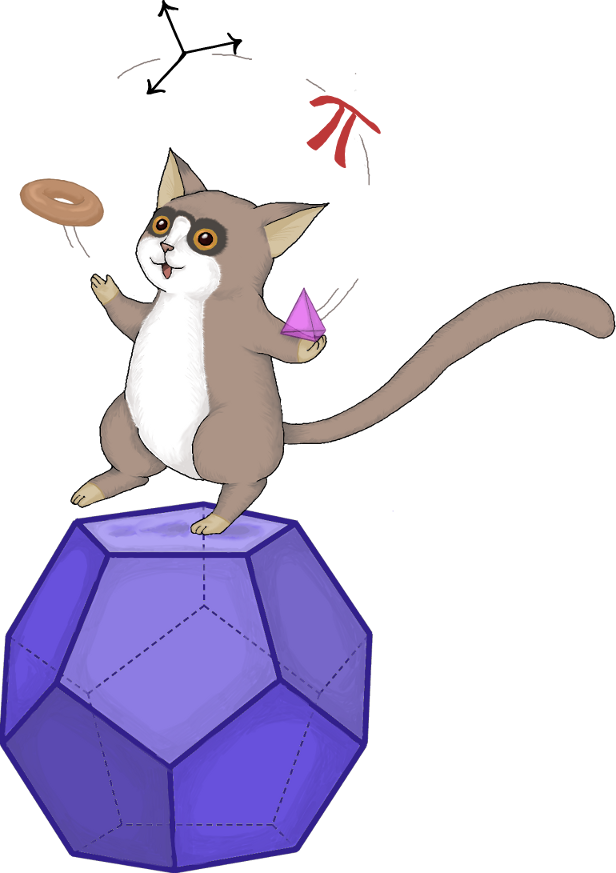
\includegraphics[scale=0.17]{cover}
}
\end{picture} 
	
\vspace{6em}

\section*{Erste Beweise mit Induktion - Lösungshinweise}

Dieses Skript enthält Lösungs\emph{hinweise} zum letzten Korrespondenzbrief. Manchmal sind dies schon die kompletten Lösungen der Aufgaben, meistens sind es aber nur einige Hinweise, die dir dabei helfen sollen, auch die Aufgaben lösen zu können, bei denen du bisher nicht weiter gekommen bist. Wenn du noch weitere Fragen zu den Aufgaben hast, kannst du uns diese weiterhin gerne per E-Mail stellen.

Wenn du uns bereits deine eigenen Lösungsversuche geschickt hast (oder noch schicken wirst - das ist selbstverständlich immer noch möglich), dann versuchen wir natürlich auch dir mit unseren Korrekturen beim Verständnis der Aufgaben zu helfen. Es lohnt sich also uns deine Lösungen zu senden :-)

%\begin{aufgabe}{Der nächste Schritt}
%	\missingfigure{Bild des fünften Schrittes}
%\end{aufgabe}
\addtocounter{aufgabennummer}{1}

\begin{aufgabe}{Wie viele neue Münzen?}\label{aufg:ZusMuenzenInViereck}
	Man benötigt $4\cdot n$ zusätzliche Münzen - nämlich für jede der vier Seiten des Quadrates $n$ Stück.
\end{aufgabe}

\begin{aufgabe}{Zentrierte Dreieckszahl}
	Wir zeigen: Die $n$-te zentrierte Dreieckszahl ist $1$ mehr als eine durch $3$ teilbare Zahl:
	
	\begin{description}
		\item[IA ($n=1$):] Das erste Dreieck besteht nur aus einer einzigen Münze. Und $1$ ist $1$ mehr als eine durch $3$ teilbare Zahl (nämlich $0$).
		\item[IV (festes $n$):] Wir haben ein Dreieck mit Seitenlänge $n$, für das wir bereits wissen, dass die Zahl der dafür nötigen Münzen $x$ eins mehr ist als eine durch $3$ teilbare Zahl. Oder anders gesagt: $x-1$ \emph{ist} durch $3$ teilbar.
		\item[IS ($n\to n+1$):] Wir nehmen das Dreieck mit Seitenlänge $n$ und machen daraus eines mit Seitenlänge $n+1$, indem wir an jeder Seite eine zusätzliche Reihe Münzen dazulegen. Dazu benötigen wir $3\cdot n$ Münzen. Also haben wir nun insgesamt $x + 3n$ Münzen verwendet und $(x+3n)-1 = (x-1)+3n$ ist durch $3$ teilbar.
	\end{description}
\end{aufgabe}


\begin{aufgabe}{Eine Summenformel}
	\begin{description}
	\item[IA ($n=1$):] Es gilt:
		\[1 = 1+3\cdot 0 = 1 + 3\cdot\frac{(1-1)\cdot 1}{2}\]
	\item[IV (festes $n$):] Es gelte bereits:
		\[1 + 1\cdot3 + 2\cdot3 + \dots + (n-1)\cdot 3 = 1 + 3\cdot\frac{(n-1)\cdot n}{2}\] 
	\item[IS ($n\to n+1$):] Mit Hilfe der Induktionsvoraussetzung (IV) zeigen wir:
		\begin{align*}
			&1 + 1\cdot3 + 2\cdot3 + \dots + (n-1)\cdot 3 + (n+1-1)\cdot 3 = \\
			=&  \left(1 + 1\cdot3 + 2\cdot3 + \dots + (n-1)\cdot 3\right) + n\cdot 3 = \\
			\overset{\text{IV}}{=}& 1 + 3\cdot\frac{(n-1)\cdot n}{2} + n\cdot 3 = \\
			=& 1 + 3\cdot \frac{(n-1)\cdot n + 2n}{2} = \\
			=& 1 + 3\cdot \frac{n^2 - n + 2n}{2} = \\
			=& 1 + 3\cdot \frac{n^2 + n}{2} = \\
			=& 1 + 3\cdot\frac{n\cdot (n+1)}{2} = \\
			=& 1 + 3\cdot\frac{((n+1)-1)\cdot (n+1)}{2}
		\end{align*} 
	\end{description}
\end{aufgabe}

\begin{aufgabe}{Déjà-vu}\label{aufg:dejavu}
	$2n^2-2n+1$ ist die Zahl der Münzen im $n$-ten zentrierten Viereck. Wir können dies zum Beispiel durch Induktion zeigen:
	
	\begin{description}
		\item[IA ($n=1$):] $2n^2-2n+1  = 2\cdot 1^2 -2 \cdot 1 + 1= 1$ und tatsächlich besteht das erste zentrierte Viereck aus genau einer Münze.
		\item[IV (festes $n$):] Für festes $n$ sei $2n^2-2n+1$ die Zahl der Münzen im $n$-ten Viereck.
		\item[IS ($n \to n+1$):] Wir wissen bereits (durch die Induktionsvoraussetzung), dass das $n$-te Viereck aus $2n^2 -2n +1$ Münzen besteht. Um daraus das $(n+1)$-te Viereck zu erhalten benötigen wir nach Aufgabe \ref{aufg:ZusMuenzenInViereck} zusätzliche $4(n+1)$ Münzen. Insgesamt besteht das $(n+1)$-te Viereck damit aus
		\[2n^2-2n+1 + 4(n+1) = 2n^2 +2n +5 = 2(n^2 + 2n +1) -2n+3 = 2(n+1)^2 - 2(n+1) +1\]
		Münzen - was genau die behauptete Aussage für $n+1$ ist.
	\end{description}
	
	$1 + 3\cdot\frac{(n-1)\cdot n}{2}$ ist die Zahl der Münzen im $n$-ten zentrierten Dreieck. Beweisen kann man das völlig analog zum obigen Beweis.
\end{aufgabe}

\begin{aufgabe}{Induktion oder Nicht-Induktion?}
	Durch Termumformung:
		\[2n^2-2n+1 = n^2 + n^2-2n+1 = n^2 + (n-1)^2\]
		
	Ein Induktionsbeweis ist hier umständlicher als notwendig - möglich ist er aber trotzdem:
	\begin{description}
		\item[IA ($n=1$):] $2n^2-2n+1  = 2\cdot 1^2 -2 \cdot 1 + 1= 1 = 1^2 + 0^2$.
		\item[IV (festes $n$):] Für festes $n$ sei $2n^2-2n+1 = n^2 + (n-1)^2$.
		\item[IS ($n \to n+1$):] Es gilt:
			\begin{align*}
				(n+1)^2 + (n+1-1)^2 &= n^2 + 2n + 1 + n^2 = n^2-2n +1 + 4n + n^2 = (n-1)^2 + 4n + n^2 \\ 
				&=n^2 + (n-1)^2 + 4n \overset{\text{IV}}{=} 2n^2 - 2n + 1 + 4n \\
				&= 2(n^2 + 2n + 1) -2 -6n + 1 + 4n = 2(n+1)^2 - 2(n+1) + 1
			\end{align*}
	\end{description}	
\end{aufgabe}


\begin{aufgabe}{Ein flächenloses Dreieck}
	\begin{description}
		\item[IA:] Im ersten Schritt verliert das Dreieck ein Viertel seiner Fläche - übrig bleiben also noch $\frac{3}{4}\cdot \SI{4}{\cm\squared} = \SI{3}{\cm\squared} = \frac{9}{1+2}\,\si{\cm\squared}$.
		\item[IV:] Nach dem $n$-ten Schritt habe das Dreieck noch eine Fläche von $\frac{9}{n+2}$ \si{\cm\squared} oder weniger.
		\item[IS:] Nach einem weiteren Schritt (dem $(n+1)$-ten), beträgt die graue Fläche noch:
			\begin{align*}
			\frac{3}{4}\cdot\frac{9}{n+2}\,\si{\cm\squared} &= \frac{27}{4(n+2)}\,\si{\cm\squared} = \frac{27}{4n+8}\,\si{\cm\squared} = \frac{27}{3n+n+8}\,\si{\cm\squared} \leq \\
			&\leq \frac{27}{3n+1+8}\,\si{\cm\squared} = \frac{27}{3n+9}\,\si{\cm\squared} = \frac{9}{(n+1)+2}\,\si{\cm\squared}
			\end{align*}
		\end{description}
\end{aufgabe}

\begin{aufgabe}{Einige Beispiele}\label{aufgabe:JosephusBspe}
	\begin{center}
		\renewcommand{\arraystretch}{2}\setlength{\tabcolsep}{1em}
		\begin{tabular}{l||c|c|c|c|c|c|c|c|c}
			Gruppengröße:	& 2	& 3 & 4 & 5 & 6 & 7 & 8 & 11 & 16 \\\hline
			Letzte Person:	& 0 & 2 & 0 & 2 & 4 & 6 & 0 & 6  & 0  
		\end{tabular}
	\end{center}
\end{aufgabe}

\begin{aufgabe}{Das Josephus-Problem für $2$er-Potenzen}\label{aufg:JosephusZweierPotenz}
Der Beweis mit gefüllten Lücken:
\begin{proof}
	Wir beweisen den Satz durch Induktion über $n$:
	\begin{description}
		\item[IA ($n=1$):] Bei einer Gruppengröße von $2^1=2$ Personen ist lediglich ein einziger Spielzug notwendig: Spieler $0$ beginnt, indem er Spieler $1$ antippt. Dieser scheidet aus, wodurch Spieler $0$ als letzter Spieler übrig bleibt.
		\item[IV:] Wir wissen für festes $n$: Bei einer Gruppe mit $2^n$ Personen bleibt am Ende der Spieler $0$ übrig.
		\item[IS ($n\to n+1$):] Wir haben nun also eine Gruppe aus $2^{n+1} = 2\cdot 2^n$ Spielern und wollen erneut zeigen, dass am Ende der Spieler $0$ übrig bleibt. Dazu starten wir das Verfahren und stoppen es, sobald zum ersten Mal wieder der Spieler $0$ an der Reihe ist. Folgende Spieler sind jetzt noch übrig:
		\[0, \underline{2}, \underline{4}, \underline{6}, \underline{8}, \dots , \underline{2^{n+1}-2}\]
		Also gerade alle Spieler mit einer \underline{geraden} Nummer. Teilen wir jetzt die Nummer jedes verbliebenen Spielers durch $2$, so sind wir in der Anfangssituation des Abzählverfahrens für eine Gruppe mit \underline{$2^n$} Spielern. Und für eine solche Gruppe wissen wir wegen der Induktionsvoraussetzung bereits, welcher Spieler am Ende übrig bleibt - nämlich Spieler \underline{$0$}. \qedhere
	\end{description}
\end{proof}
\end{aufgabe}

\begin{aufgabe}{Wer bleibt übrig?}
	Besteht die Gruppe aus $2^n + k$ Personen, so lassen wir sie zunächst die ersten $k$ Spielzüge durchführen. Nach diesen besteht die Gruppe nur noch aus $2^n$ Spielern und der $(2k)$-te Spieler ist an der Reihe\footnote{Wir sollten hier also annehmen, dass $k < 2^n$ gilt. Warum können wir das machen ohne dadurch wieder irgendwelche Fälle zu vergessen?}. 
	
	Für eine solche Spielsituation haben wir aber bereits in Aufgabe \ref{aufg:JosephusZweierPotenz} gezeigt, welcher Spieler das Spiel gewinnt: Nämlich der Spieler, der zu Beginn an der Reihe ist.
	
	Insgesamt haben wir damit also gezeigt, dass bei einer Gruppe aus $2^n + k$ (mit $k < 2^n$) Spielern am Ende der $(2k)$-te Spieler übrig bleibt.
\end{aufgabe}

\begin{aufgabe}{Zur Kontrolle}
	\begin{center}
		\renewcommand{\arraystretch}{2}\setlength{\tabcolsep}{1em}
		\begin{tabular}{l||c|c|c|c|c|c|c|c}
			Gruppengröße:	& 32 & 35 & 41 & 64 & 130 & 512 & 1025 & 2047 \\\hline
			Letzte Person:	& 0  & 6  & 18 & 0  & 4   & 0   & 2    & 2046    
		\end{tabular}
	\end{center}	
\end{aufgabe}



\end{document}